\section{Простір професійного розвитку}

\subsection{Структура курсу}

Не те, щоб це була якась новина, впевнені багато
хто дотримується такої карти топового програміста,
але я візьму на собі сміливість відкрити це таємне
знання. Почну опис курсу з відомої мемної картинки.


\subsection{Дракон}

Юнікорнами називають тих програмістів, які однаково
добре володіють CSS скажімо, а також можуть повністю
побудувати будь-якої складності тонкий чи товстий
клієнт не обмежуючись HTML5, а й переходячи у SVG
чи WPF, чи DirectX чи OpenGL.

Фулстек програмістами називають фахівців із
побудови інформаційних систем на кордоні з
єдинорогами (які зазвичай не займаються процесиногом,
інфраструктурою, мережами та захистом).

\begin{figure}[!htbp]
\centerline{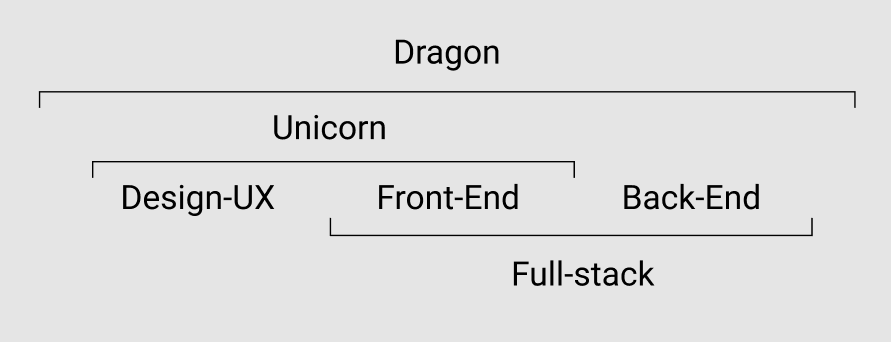
\includegraphics[scale=0.35]{dragon.PNG}}
\caption{Дракон}
\end{figure}

\subsection{Лямбдагарбха}

Наступний рівень -- це платформоутворюючий рівень,
який включає мову програмування, рантайм та апаратуру.
Зазвичай дорослі академічні мови створюються відразу з
рантаймом, тому назвемо цю секцію рівень університетського
професора, а секцію рантайму (ОС) та апаратура назвемо
підприємницької, оскільки ОС зазвичай продають разом
із залізом і всі, хто це намагався просувати на ринок,
можна прирівняти до бодхісатств. Останні відомі лямбдагарбхи ---
це давні автори перших Лісп машин та XEROX PARC.

\begin{figure}[!htbp]
\centerline{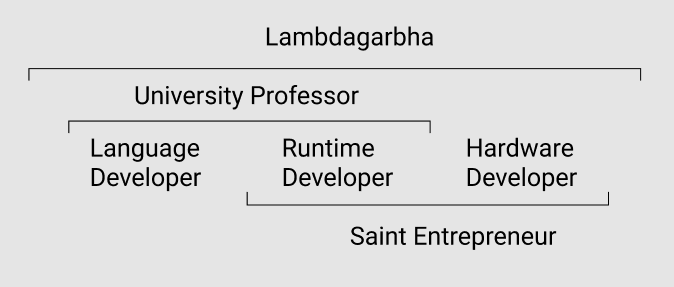
\includegraphics[scale=0.46]{lambdagarbha.PNG}}
\caption{Лямбдагарбха}
\end{figure}

\newpage
\subsection{Гротендік}

На абсолютном уровне программисты (в том числе и топовые) являются математиками, поэтому тут можно отметить ядро которое было открыто Квилленом — модельные категории, в которых работали не только медалисты Филдса — Воеводский и сам Квиллен, но которые являются также основным инструментом современных теоретико-типовых математиков как Шульман. Предмет изучающий модельные категории Квиллен назвал гомотопической алгеброй, при помощи которой была построена не только модель алгебраической топологии самим Квилленом, но и А1-теория гомотопий Воеводского. Все это крышуется Гротендиком, как мультидисциплинарным программистом абсолютного уровня (топ-математиком).

\begin{figure}[!htbp]
\centerline{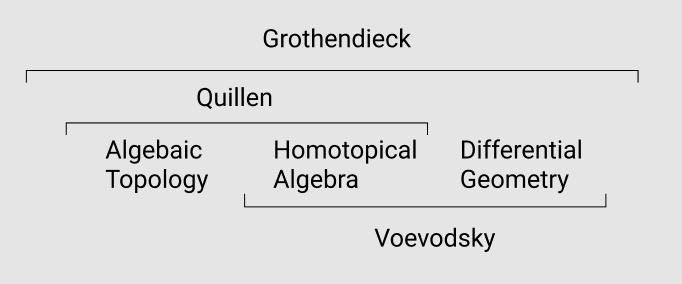
\includegraphics[scale=0.46]{grothendieck.PNG}}
\caption{Гротендік}
\end{figure}

\newpage
\subsection{Будда}

Без лишней скромности, любой программист который смог не только представить, но и успеть порабать за жизнь на всех уровнях, может считать себя Буддой программирования, или как мы скромно называем таких пацанов — хуй с горы.

\begin{figure}[!htbp]
\centerline{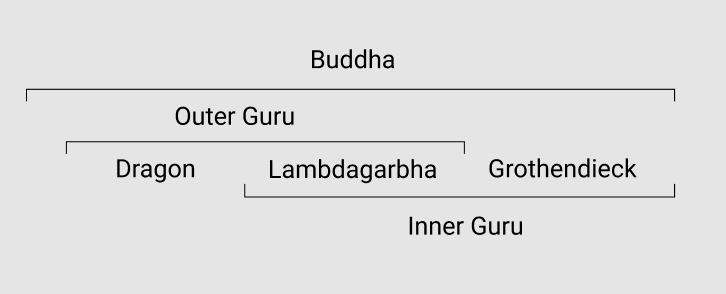
\includegraphics[scale=0.46]{buddha.PNG}}
\caption{Будда}
\end{figure}

\normalsize
